\section{Deployments: (How) Is Feedback Reused?}
To understand how feedback is reused in educational settings and evaluate the CritiqueKit approach, we conducted two deployments and two experiments. All studies took place at a research university. 

\subsection{DEP 1: How Do Teaching Assistants Reuse Feedback?}
Eight teaching assistants (TAs) (two female) for an undergraduate design course used Gradescope to grade and critique seven weekly assignments that varied in content from storyboards to written explanations to high-fidelity web application prototypes. TAs set rubric items for each assignment and wrote comments for each. We deployed CritiqueKit to first understand how TAs might reuse feedback and made iterative improvements to the design throughout the quarter based on TA input.

\begin{figure}[b!]
\centering
  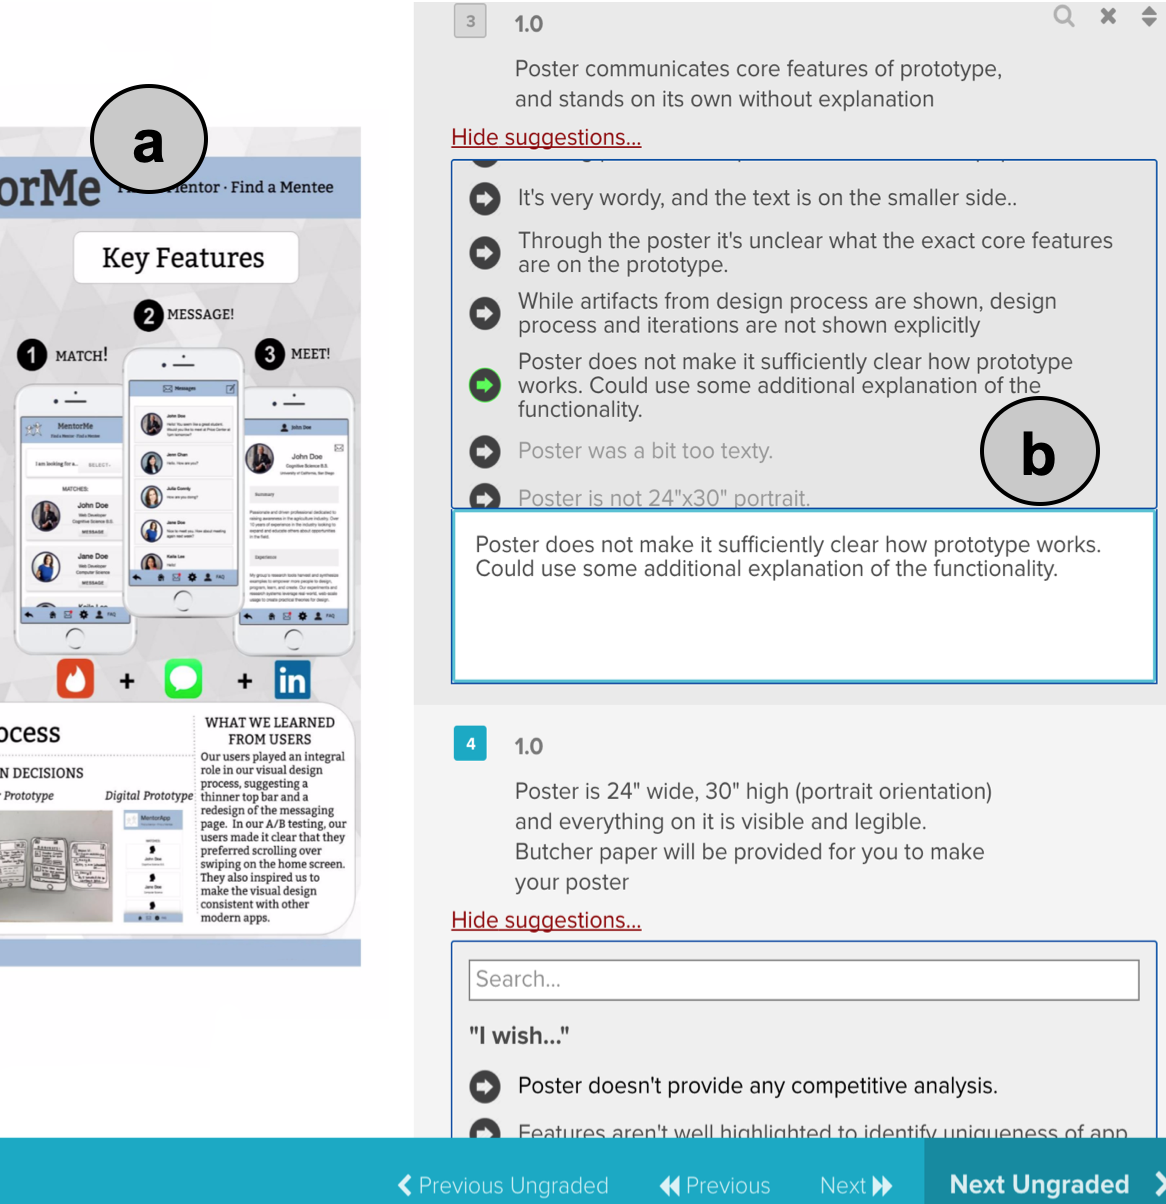
\includegraphics[width=0.6\textwidth]{critiquekit/figures/gradescope.png}
  \caption{CritiqueKit implemented as a browser extension in Gradescope for DEP 1. a) Reviewers provide feedback on a student design. b) The suggestions box under each rubric item provides reviewers with a list of reusable suggestions and a comment box for providing feedback on a submission.}~\label{fig:critiquekit_gradescope}
\end{figure}

\subsubsection{Method: Integrating CritiqueKit with Gradescope}
To integrate with the TAs' existing workflow, we implemented CritiqueKit as a Google Chrome extension that augments the Gradescope interface with a suggestions box (\autoref{fig:critiquekit_gradescope}). This version of CritiqueKit contained only the suggestions box to explore feedback reuse. The suggestions box contained a manually curated set of feedback provided by former TAs in a previous iteration of the course, stored in a Google Sheet online and retrieved by the Chrome extension using the Google Sheets API. Suggestions were categorized into three feedback categories: Positive, Problem, and Solution. TAs could select feedback suggestions to directly copy into the textbox for further editing. Each rubric item contained its own suggestion box interface, providing suggestions specific to that rubric item.

We curated the reusable suggestions corpus as follows. Given all feedback from the previous quarter, feedback that was 25 or fewer words in length was kept, because longer feedback was both too long to be skimmed in a suggestion display and tended to be overly specific. Feedback of 26-30 words was truncated at the sentence level to fit within the 25-word limit. Longer comments or duplicate comments were discarded. In total, 526 comments were provided as suggestions throughout the course for seven (of ten) assignments. Suggestions were manually categorized into the Positive ($n = 92$), Problem ($n = 312$), and Solution ($n = 122$) categories.

\subsubsection{Result: TAs Used Feedback Suggestions as Inspiration}
Across seven assignments, four of the eight TAs reused 51 distinct suggestions from the 526-element corpus (9.7\%). 75 of 583 designs received a reused suggestion for feedback. 60\% of reused suggestions were categorized in the Problem category. These numbers omit any reuse occurring entirely inside Gradescope without CritiqueKit. (Gradescope provides an interface for reusing entire comments within an assignment rather than for individual parts of the comment.) 

An end-of-course survey asked TAs about their CritiqueKit use. One commented that he would ``\textit{skim the comments in the [suggestions] to see if something was accurate to my thoughts}.'' Another mentioned that the prototype helped him ``\textit{[find] ways to better explain and give feedback about specific points}.'' TAs also mentioned that suggestions sometimes reminded them to comment on more diverse aspects of students' work. For example, one mentioned that seeing positive suggestions reminded her to give positive feedback, not only critiquing areas for improvement. TAs mentioned using the suggestions as inspiration rather than the exact wording, taking the underlying concept of a suggestion and tailoring it.

\subsection{DEP 2: How Do Students Reuse Feedback?}
The first deployment examined teaching staff usage; this second deployment examined student usage to understand how novices interact with guidance and suggestions. We deployed CritiqueKit as a standalone web application with 29 students in an undergraduate design course for five weeks. Students gave anonymous feedback on two randomly assigned peer submissions for each of seven assignments.

\begin{figure}[b!]
\centering
  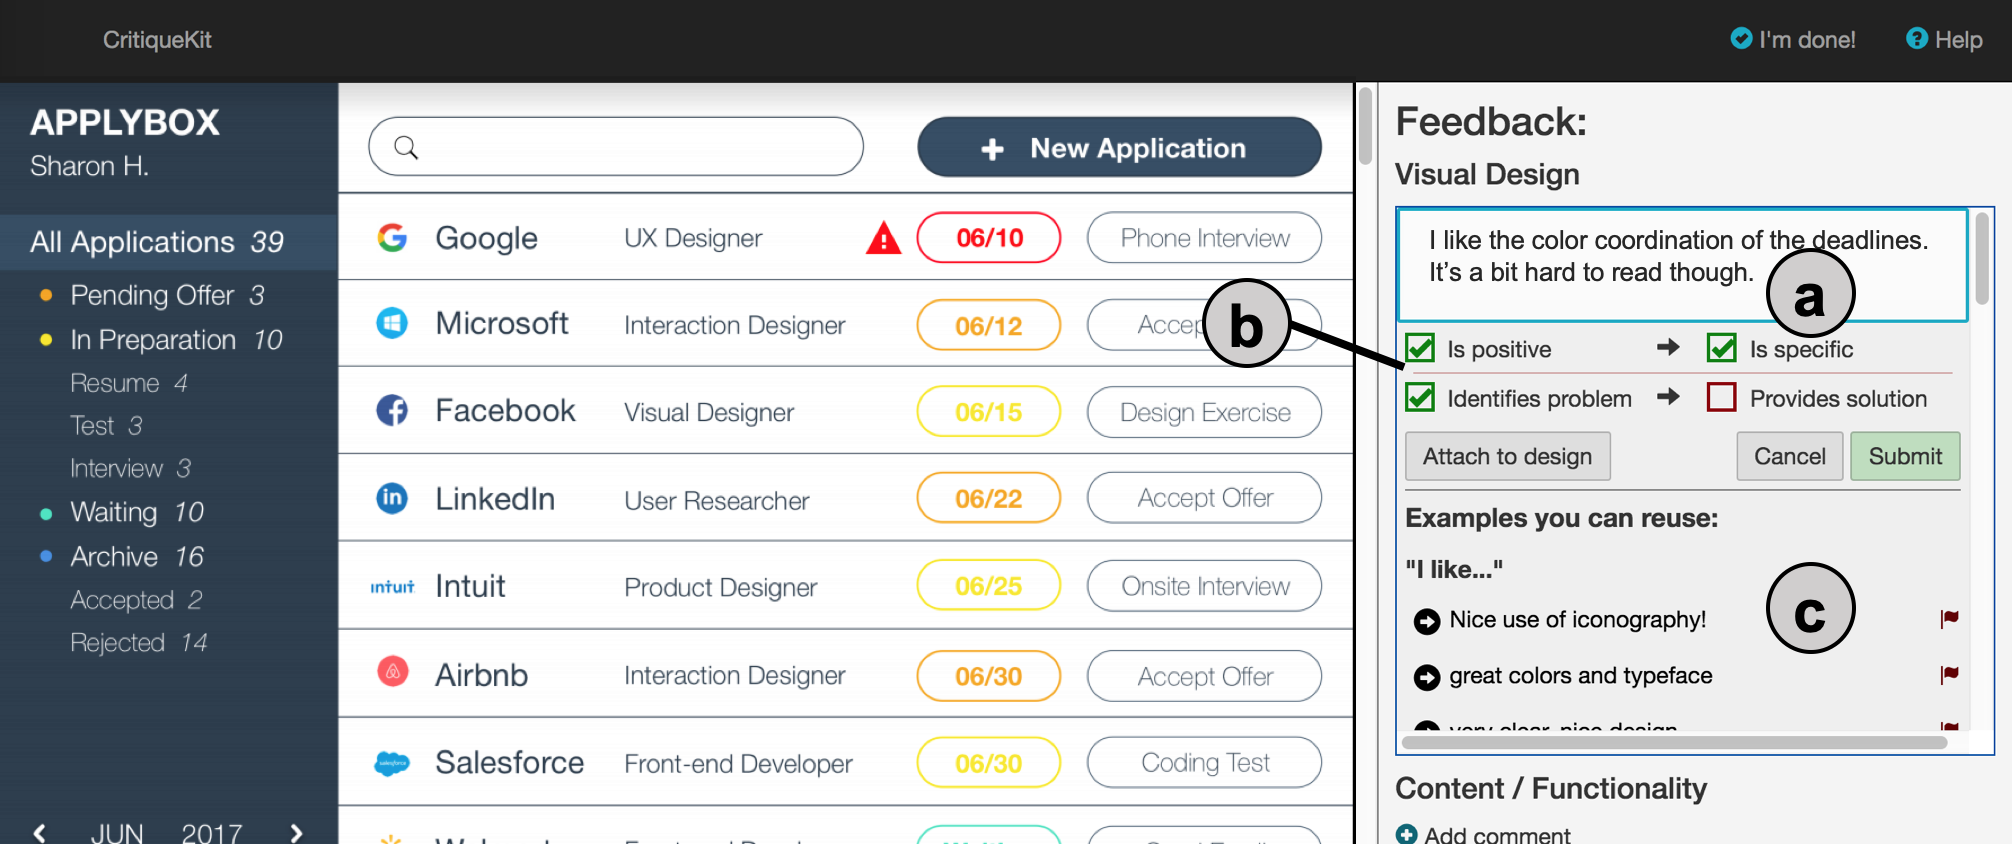
\includegraphics[width=\textwidth]{critiquekit/figures/old_interface.png}
  \caption[The CritiqueKit user interface for DEP 2 and EXP 1.]{The CritiqueKit user interface for DEP 2 and EXP 1. a) The reviewer types their feedback into the text box. b) Checkboxes in the guidance panel update as the reviewer types to show how well the comment fulfills high-quality feedback criteria. c) The reviewer can browse and reuse previously given feedback.}~\label{fig:critiquekit_exp1}
\end{figure}

\subsubsection{Method: Integrating Interactive Guidance for Scaffolding}
Novice students are less experienced in giving feedback and may benefit from interactive scaffolding \cite{Reiser2004}. This version of CritiqueKit included an interactive guidance panel to help reviewers provide more specific and actionable feedback (\autoref{fig:critiquekit_exp1}). The categories on the guidance panel were ``Is Positive,'' ``Is Specific,'' ``Identifies a Problem,'' and ``Presents a Solution'' with checkboxes next to each. These categories stem from recommendations in the literature for both positive and critical feedback \cite{Kelley2013}. Similar to the final version of CritiqueKit, these checkboxes updated as a reviewer typed by classifying their comment into the three categories. The categories differed from the final version, focusing on specific and actionable feedback. 

The suggestions box was seeded with feedback from the course TA. Similar to the first deployment, the suggestions were categorized in the Positive, Problem, and Solution categories. When a student submitted a comment, it was classified into one of these categories, shortened to 25 words if it was longer, and fed back into the corpus to appear as a suggestion, enabling students to reuse their peers' as well as their own comments. The suggestions were ordered first by frequency used, then by shortest length first, and updated as these values changed and more comments were added. Compared to the final version of CritiqueKit, suggestions were static, meaning they did not change as the reviewer typed.

\subsubsection{Results: Positive Feedback Common; Reuse Rare}
For seven assignments, 898 comments were submitted. Independent raters classified each comment into the five categories of Positive Only, Positive  and  Specific (Positive + Specific), Problem Only, Solution Only, and Problem with a Solution (Problem + Solution). 45\% of these comments contained positive feedback; 30\% contained a Problem + Solution statement. 

Students rarely selected feedback suggestions for reuse. Over the five-week deployment, 14 distinct suggestions were reused on 27 student designs for four of the seven assignments. These suggestions were mostly short, vague comments such as ``I wish this was more visually appealing.'' This may be because students often left feedback specific to individual designs that did not easily generalize to other contexts. Students' comments in a post-survey confirmed that the suggestions did not always seem applicable. Students also did not regularly use the interactive guidance panel; 15 of the 29 students engaged with the panel a total of 120 times over five weeks. 

In contrast to how TAs reused feedback, students may not have recognized common issues. TAs paid attention to common errors between designs and mainly reused Problem feedback, whereas students may not have noticed or attended to underlying issues between designs. For instance, one student mentioned that they did not use the feedback suggestions because they ``\textit{rarely pointed out the same things when critiquing interfaces}.'' 

This exploratory deployment investigated how students reuse feedback and respond to interactive guidance in the classroom. To understand how a system with these features compares to a standard feedback system, the next study was a controlled between-subjects experiment. 
